\INEchaptercarta{Gasto de los hogares}{}

\cajita{Gasto en educación}{El gasto promedio en educación per cápita\llamada en 2014 tuvo una disminución del 8.78\%\llamada respecto al de 2011.\textollamada{El indicador se calcula por persona, y no por hogar, debido a la amplitud del número de miembros de los hogares.}
	
	\textollamada{Los cálculos están realizados en quetzales corrientes de cada año.} }{Gasto promedio anual per cápita en educación}{República de Guatemala, serie histórica por Encovi, en quetzales de cada año}{\ \\[0mm]\begin{tikzpicture}[x=1pt,y=1pt]  % Created by tikzDevice version 0.9 on 2016-02-28 22:06:14
% !TEX encoding = UTF-8 Unicode
\definecolor{fillColor}{RGB}{255,255,255}
\path[use as bounding box,fill=fillColor,fill opacity=0.00] (0,0) rectangle (289.08,198.74);
\begin{scope}
\path[clip] (  0.00,  0.00) rectangle (289.08,198.74);

\path[] (  0.00,  0.00) rectangle (289.08,198.74);
\end{scope}
\begin{scope}
\path[clip] (  0.00,  0.00) rectangle (289.08,198.74);

\path[] (  3.86, 15.61) rectangle (280.54,191.48);

\path[] (  3.86, 43.22) --
	(280.54, 43.22);

\path[] (  3.86, 82.44) --
	(280.54, 82.44);

\path[] (  3.86,121.67) --
	(280.54,121.67);

\path[] (  3.86,160.90) --
	(280.54,160.90);

\path[] (  3.86, 23.61) --
	(280.54, 23.61);

\path[] (  3.86, 62.83) --
	(280.54, 62.83);

\path[] (  3.86,102.06) --
	(280.54,102.06);

\path[] (  3.86,141.28) --
	(280.54,141.28);

\path[] (  3.86,180.51) --
	(280.54,180.51);

\path[] ( 43.39, 15.61) --
	( 43.39,191.48);

\path[] (109.26, 15.61) --
	(109.26,191.48);

\path[] (175.14, 15.61) --
	(175.14,191.48);

\path[] (241.02, 15.61) --
	(241.02,191.48);
\definecolor{drawColor}{RGB}{0,0,255}

\path[draw=drawColor,line width= 1.7pt,line join=round] ( 43.39, 86.31) --
	(109.26,142.26) --
	(175.14,183.49) --
	(241.02,169.44);
\definecolor{drawColor}{RGB}{0,0,0}

\node[text=drawColor,anchor=base,inner sep=0pt, outer sep=0pt, scale=  1.02] at ( 43.39, 74.40) {319.7};

\node[text=drawColor,anchor=base east,inner sep=0pt, outer sep=0pt, scale=  1.02] at (105.25,142.26) {605.0};

\node[text=drawColor,anchor=base,inner sep=0pt, outer sep=0pt, scale=  1.02] at (175.14,187.46) {815.2};

\node[text=drawColor,anchor=base,inner sep=0pt, outer sep=0pt, scale=  1.02] at (241.02,157.53) {743.6};

\path[draw=drawColor,line width= 0.1pt,line join=round] (  3.86, 23.61) -- (280.54, 23.61);

\path[] (  3.86, 15.61) rectangle (280.54,191.48);
\end{scope}
\begin{scope}
\path[clip] (  0.00,  0.00) rectangle (289.08,198.74);

\path[] (  3.86, 15.61) --
	(  3.86,191.48);
\end{scope}
\begin{scope}
\path[clip] (  0.00,  0.00) rectangle (289.08,198.74);

\path[] (  1.11, 23.61) --
	(  3.86, 23.61);

\path[] (  1.11, 62.83) --
	(  3.86, 62.83);

\path[] (  1.11,102.06) --
	(  3.86,102.06);

\path[] (  1.11,141.28) --
	(  3.86,141.28);

\path[] (  1.11,180.51) --
	(  3.86,180.51);
\end{scope}
\begin{scope}
\path[clip] (  0.00,  0.00) rectangle (289.08,198.74);

\path[] (  3.86, 15.61) --
	(280.54, 15.61);
\end{scope}
\begin{scope}
\path[clip] (  0.00,  0.00) rectangle (289.08,198.74);

\path[] ( 43.39, 12.86) --
	( 43.39, 15.61);

\path[] (109.26, 12.86) --
	(109.26, 15.61);

\path[] (175.14, 12.86) --
	(175.14, 15.61);

\path[] (241.02, 12.86) --
	(241.02, 15.61);
\end{scope}
\begin{scope}
\path[clip] (  0.00,  0.00) rectangle (289.08,198.74);
\definecolor{drawColor}{RGB}{0,0,0}

\node[text=drawColor,anchor=base,inner sep=0pt, outer sep=0pt, scale=  1.00] at ( 43.39,  2.85) {2000};

\node[text=drawColor,anchor=base,inner sep=0pt, outer sep=0pt, scale=  1.00] at (109.26,  2.85) {2006};

\node[text=drawColor,anchor=base,inner sep=0pt, outer sep=0pt, scale=  1.00] at (175.14,  2.85) {2011};

\node[text=drawColor,anchor=base,inner sep=0pt, outer sep=0pt, scale=  1.00] at (241.02,  2.85) {2014};
\end{scope}
  \end{tikzpicture}}{Instituto Nacional de Estadística, Encovi 2000, 2006, 2011 y 2014}

\cajita{Proporción de gasto en educación}{El gasto de los hogares en educación, como proporción del gasto total tuvo en el 2014 un  aumento de 0.9 puntos porcentuales respecto al 2006 pero en 2014 registró una baja de 1.9 puntos. }{Gasto en educación como proporción del gasto total}{República de Guatemala, serie histórica por Encovi, en porcentaje}{\ \\[0mm]\begin{tikzpicture}[x=1pt,y=1pt]  % Created by tikzDevice version 0.9 on 2016-02-28 22:06:17
% !TEX encoding = UTF-8 Unicode
\definecolor{fillColor}{RGB}{255,255,255}
\path[use as bounding box,fill=fillColor,fill opacity=0.00] (0,0) rectangle (289.08,198.74);
\begin{scope}
\path[clip] (  0.00,  0.00) rectangle (289.08,198.74);

\path[] (  0.00,  0.00) rectangle (289.08,198.74);
\end{scope}
\begin{scope}
\path[clip] (  0.00,  0.00) rectangle (289.08,198.74);

\path[] ( -4.90, 15.61) rectangle (280.54,191.48);

\path[] (  0.00, 46.12) --
	(280.54, 46.12);

\path[] (  0.00, 91.16) --
	(280.54, 91.16);

\path[] (  0.00,136.20) --
	(280.54,136.20);

\path[] (  0.00,181.24) --
	(280.54,181.24);

\path[] (  0.00, 23.61) --
	(280.54, 23.61);

\path[] (  0.00, 68.64) --
	(280.54, 68.64);

\path[] (  0.00,113.68) --
	(280.54,113.68);

\path[] (  0.00,158.72) --
	(280.54,158.72);

\path[] ( 35.88, 15.61) --
	( 35.88,191.48);

\path[] (103.84, 15.61) --
	(103.84,191.48);

\path[] (171.80, 15.61) --
	(171.80,191.48);

\path[] (239.77, 15.61) --
	(239.77,191.48);
\definecolor{drawColor}{RGB}{0,0,255}

\path[draw=drawColor,line width= 1.7pt,line join=round] ( 35.88,140.70) --
	(103.84,163.22) --
	(171.80,183.49) --
	(239.77,140.70);
\definecolor{drawColor}{RGB}{0,0,0}

\node[text=drawColor,anchor=base,inner sep=0pt, outer sep=0pt, scale=  1.02] at ( 35.88,128.79) {5.2};

\node[text=drawColor,anchor=base east,inner sep=0pt, outer sep=0pt, scale=  1.02] at (101.60,163.22) {6.2};

\node[text=drawColor,anchor=base,inner sep=0pt, outer sep=0pt, scale=  1.02] at (171.80,187.46) {7.1};

\node[text=drawColor,anchor=base,inner sep=0pt, outer sep=0pt, scale=  1.02] at (239.77,128.79) {5.2};

\path[draw=drawColor,line width= 0.1pt,line join=round] (  0.00, 23.61) -- (280.54, 23.61);

\path[] ( -4.90, 15.61) rectangle (280.54,191.48);
\end{scope}
\begin{scope}
\path[clip] (  0.00,  0.00) rectangle (289.08,198.74);

\path[] (  0.00, 15.61) --
	(280.54, 15.61);
\end{scope}
\begin{scope}
\path[clip] (  0.00,  0.00) rectangle (289.08,198.74);

\path[] ( 35.88, 12.86) --
	( 35.88, 15.61);

\path[] (103.84, 12.86) --
	(103.84, 15.61);

\path[] (171.80, 12.86) --
	(171.80, 15.61);

\path[] (239.77, 12.86) --
	(239.77, 15.61);
\end{scope}
\begin{scope}
\path[clip] (  0.00,  0.00) rectangle (289.08,198.74);
\definecolor{drawColor}{RGB}{0,0,0}

\node[text=drawColor,anchor=base,inner sep=0pt, outer sep=0pt, scale=  1.00] at ( 35.88,  2.85) {2000};

\node[text=drawColor,anchor=base,inner sep=0pt, outer sep=0pt, scale=  1.00] at (103.84,  2.85) {2006};

\node[text=drawColor,anchor=base,inner sep=0pt, outer sep=0pt, scale=  1.00] at (171.80,  2.85) {2011};

\node[text=drawColor,anchor=base,inner sep=0pt, outer sep=0pt, scale=  1.00] at (239.77,  2.85) {2014};
\end{scope}
  \end{tikzpicture}}{Instituto Nacional de Estadística, Encovi 2000, 2006 y 2011}


%aquí va la nueva 32.3


\cajita{Gasto en educación según jefatura del hogar}{El gasto de los hogares en educación muestra diferencias según el sexo de la persona que es jefe de hogar. Hasta 2011 ambas tendencias mostraron crecimiento, sin embargo, para el año 2014 se registró una baja en el gasto de educación respecto del gasto total.  Además es importante recalcar que en los hogares con jefatura mujer la asignación de gasto en educación en mayor que en los hogares con jefatura hombre.}{Proporción del gasto promedio per cápita en educación según sexo de la jefatura del hogar}{República de Guatemala, serie histórica por Encovi, en quetzales de cada año}{\ \\[0mm]\begin{tikzpicture}[x=1pt,y=1pt]  % Created by tikzDevice version 0.9 on 2016-02-28 22:06:18
% !TEX encoding = UTF-8 Unicode
\definecolor{fillColor}{RGB}{255,255,255}
\path[use as bounding box,fill=fillColor,fill opacity=0.00] (0,0) rectangle (289.08,198.74);
\begin{scope}
\path[clip] (  0.00,  0.00) rectangle (289.08,198.74);

\path[] (  0.00,  0.00) rectangle (289.08,198.74);
\end{scope}
\begin{scope}
\path[clip] (  0.00,  0.00) rectangle (289.08,198.74);

\path[] (  0.00, 18.46) rectangle (289.08,172.85);

\path[] ( 41.30, 18.46) --
	( 41.30,172.85);

\path[] (110.13, 18.46) --
	(110.13,172.85);

\path[] (178.95, 18.46) --
	(178.95,172.85);

\path[] (247.78, 18.46) --
	(247.78,172.85);
\definecolor{drawColor}{RGB}{0,0,255}
\definecolor{fillColor}{RGB}{0,0,255}

\path[draw=drawColor,line width= 0.6pt,line join=round,fill=fillColor] ( 14.63, 18.46) rectangle ( 37.00,108.52);
\definecolor{drawColor}{RGB}{157,187,255}
\definecolor{fillColor}{RGB}{157,187,255}

\path[draw=drawColor,line width= 0.6pt,line join=round,fill=fillColor] ( 45.60, 18.46) rectangle ( 67.97,117.10);
\definecolor{drawColor}{RGB}{0,0,255}
\definecolor{fillColor}{RGB}{0,0,255}

\path[draw=drawColor,line width= 0.6pt,line join=round,fill=fillColor] ( 83.45, 18.46) rectangle (105.82,125.67);
\definecolor{drawColor}{RGB}{157,187,255}
\definecolor{fillColor}{RGB}{157,187,255}

\path[draw=drawColor,line width= 0.6pt,line join=round,fill=fillColor] (114.43, 18.46) rectangle (136.80,140.68);
\definecolor{drawColor}{RGB}{0,0,255}
\definecolor{fillColor}{RGB}{0,0,255}

\path[draw=drawColor,line width= 0.6pt,line join=round,fill=fillColor] (152.28, 18.46) rectangle (174.65,168.56);
\definecolor{drawColor}{RGB}{157,187,255}
\definecolor{fillColor}{RGB}{157,187,255}

\path[draw=drawColor,line width= 0.6pt,line join=round,fill=fillColor] (183.26, 18.46) rectangle (205.63,172.85);
\definecolor{drawColor}{RGB}{0,0,255}
\definecolor{fillColor}{RGB}{0,0,255}

\path[draw=drawColor,line width= 0.6pt,line join=round,fill=fillColor] (221.11, 18.46) rectangle (243.48,123.74);
\definecolor{drawColor}{RGB}{157,187,255}
\definecolor{fillColor}{RGB}{157,187,255}

\path[draw=drawColor,line width= 0.6pt,line join=round,fill=fillColor] (252.08, 18.46) rectangle (274.45,159.12);
\definecolor{drawColor}{RGB}{0,0,0}

\path[draw=drawColor,line width= 0.6pt,line join=round] (  0.00, 18.46) -- (289.08, 18.46);

\node[text=drawColor,anchor=base,inner sep=0pt, outer sep=0pt, scale=  0.83] at ( 25.81,111.75) {4.2};

\node[text=drawColor,anchor=base,inner sep=0pt, outer sep=0pt, scale=  0.83] at ( 56.78,120.33) {4.6};

\node[text=drawColor,anchor=base,inner sep=0pt, outer sep=0pt, scale=  0.83] at ( 94.64,128.91) {5.0};

\node[text=drawColor,anchor=base,inner sep=0pt, outer sep=0pt, scale=  0.83] at (125.61,143.92) {5.7};

\node[text=drawColor,anchor=base,inner sep=0pt, outer sep=0pt, scale=  0.83] at (163.47,171.79) {7.0};

\node[text=drawColor,anchor=base,inner sep=0pt, outer sep=0pt, scale=  0.83] at (194.44,176.08) {7.2};

\node[text=drawColor,anchor=base,inner sep=0pt, outer sep=0pt, scale=  0.83] at (232.30,126.98) {4.9};

\node[text=drawColor,anchor=base,inner sep=0pt, outer sep=0pt, scale=  0.83] at (263.27,162.36) {6.6};

\path[] (  0.00, 18.46) rectangle (289.08,172.85);
\end{scope}
\begin{scope}
\path[clip] (  0.00,  0.00) rectangle (289.08,198.74);

\path[] (  0.00, 18.46) --
	(289.08, 18.46);
\end{scope}
\begin{scope}
\path[clip] (  0.00,  0.00) rectangle (289.08,198.74);

\path[] ( 41.30, 15.71) --
	( 41.30, 18.46);

\path[] (110.13, 15.71) --
	(110.13, 18.46);

\path[] (178.95, 15.71) --
	(178.95, 18.46);

\path[] (247.78, 15.71) --
	(247.78, 18.46);
\end{scope}
\begin{scope}
\path[clip] (  0.00,  0.00) rectangle (289.08,198.74);
\definecolor{drawColor}{RGB}{0,0,0}

\node[text=drawColor,anchor=base,inner sep=0pt, outer sep=0pt, scale=  1.00] at ( 41.30,  5.69) {2000};

\node[text=drawColor,anchor=base,inner sep=0pt, outer sep=0pt, scale=  1.00] at (110.13,  5.69) {2006};

\node[text=drawColor,anchor=base,inner sep=0pt, outer sep=0pt, scale=  1.00] at (178.95,  5.69) {2011};

\node[text=drawColor,anchor=base,inner sep=0pt, outer sep=0pt, scale=  1.00] at (247.78,  5.69) {2014};
\end{scope}
\begin{scope}
\path[clip] (  0.00,  0.00) rectangle (289.08,198.74);
\coordinate (apoyo) at (55.98,189.21);
\coordinate (longitudFicticia) at (7.11,9.53);
\coordinate (longitud) at (7.11,7.11);
\coordinate (desX) at (142.21,0);
\coordinate (desY) at (0,1.21);
\definecolor[named]{ct1}{HTML}{
0000FF
}
\definecolor[named]{ct2}{HTML}{
9DBBFF
}
\definecolor[named]{ctb1}{HTML}{
0000FF
}
\definecolor[named]{ctb2}{HTML}{
9DBBFF
}
\path [fill=none] (apoyo) rectangle ($(apoyo)+(longitudFicticia)$)
node [xshift=0.3cm,inner sep=0pt, outer sep=0pt,midway,right,scale = 0.9]{Hombre};
\draw [color = ctb1,fill=ct1] ( $(apoyo)  + (desY) $) rectangle ($(apoyo)+ (desY) +(longitud)$);
\path [fill=none] ($(apoyo)+(desX)$) rectangle ($(apoyo)+(desX)+(longitudFicticia)$)
node [xshift=0.3cm,inner sep=0pt, outer sep=0pt,midway,right,scale = 0.9]{Mujer};
\draw [color = ctb2 ,fill=ct2] ( $(apoyo)  + (desY) + (desX) $) rectangle ($(apoyo)+ (desY)+ (desX) +(longitud)$);
\end{scope}
  \end{tikzpicture}}{Instituto Nacional de Estadística, Encovi 2000, 2006, 2011 y 2014}


\cajita{Gasto en educación según etnicidad}{El gasto en educación de los hogares tiene diferencias según la etnicidad de la persona que es jefe de hogar.  En los hogares con jefatura indígena, la asignación de gasto fue de Q507.5 per capita. Mientras que en las jefaturas no indígenas fue de Q761.9, siendo 1.5 veces mayor que en los hogares con jefatura indígena.}{Gasto promedio per cápita anual en educación según etnicidad del jefe del hogar}{República de Guatemala, 2011, en quetzales de 2011}{\ \\[0mm]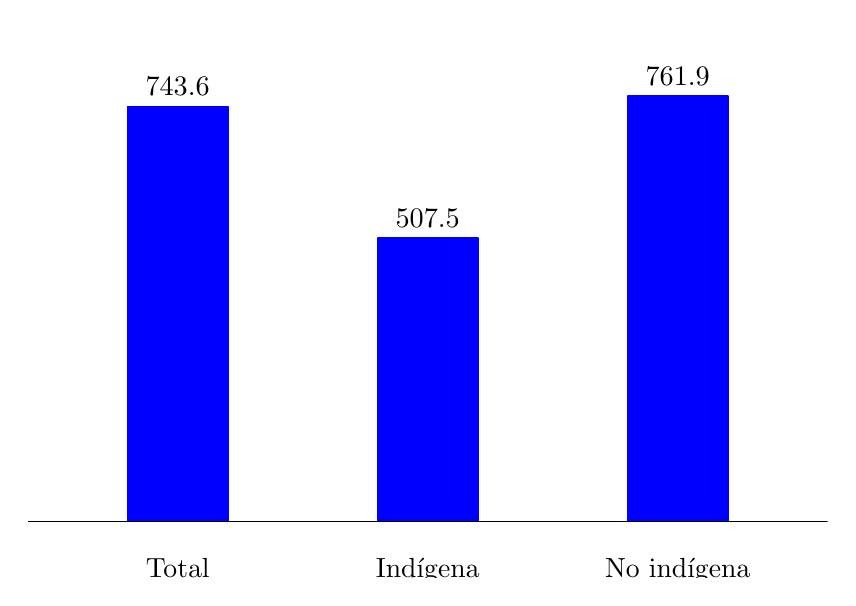
\begin{tikzpicture}[x=1pt,y=1pt]  % Created by tikzDevice version 0.9 on 2016-02-28 22:06:21
% !TEX encoding = UTF-8 Unicode
\definecolor{fillColor}{RGB}{255,255,255}
\path[use as bounding box,fill=fillColor,fill opacity=0.00] (0,0) rectangle (289.08,198.74);
\begin{scope}
\path[clip] (  0.00,  0.00) rectangle (289.08,198.74);

\path[] (  0.00,  0.00) rectangle (289.08,198.74);
\end{scope}
\begin{scope}
\path[clip] (  0.00,  0.00) rectangle (289.08,198.74);

\path[] (  0.00, 12.77) rectangle (289.08,181.67);

\path[] ( 54.20, 12.77) --
	( 54.20,181.67);

\path[] (144.54, 12.77) --
	(144.54,181.67);

\path[] (234.88, 12.77) --
	(234.88,181.67);
\definecolor{drawColor}{RGB}{0,0,255}
\definecolor{fillColor}{RGB}{0,0,255}

\path[draw=drawColor,line width= 0.6pt,line join=round,fill=fillColor] ( 36.13, 20.44) rectangle ( 72.27,170.31);

\path[draw=drawColor,line width= 0.6pt,line join=round,fill=fillColor] (126.47, 20.44) rectangle (162.61,122.73);

\path[draw=drawColor,line width= 0.6pt,line join=round,fill=fillColor] (216.81, 20.44) rectangle (252.95,173.99);
\definecolor{drawColor}{RGB}{0,0,0}

\path[draw=drawColor,line width= 0.1pt,line join=round] (  0.00, 20.44) -- (289.08, 20.44);

\node[text=drawColor,anchor=base,inner sep=0pt, outer sep=0pt, scale=  1.02] at ( 54.20,174.28) {743.6};

\node[text=drawColor,anchor=base,inner sep=0pt, outer sep=0pt, scale=  1.02] at (144.54,126.71) {507.5};

\node[text=drawColor,anchor=base,inner sep=0pt, outer sep=0pt, scale=  1.02] at (234.88,177.96) {761.9};

\path[] (  0.00, 12.77) rectangle (289.08,181.67);
\end{scope}
\begin{scope}
\path[clip] (  0.00,  0.00) rectangle (289.08,198.74);

\path[] (  0.00, 12.77) --
	(289.08, 12.77);
\end{scope}
\begin{scope}
\path[clip] (  0.00,  0.00) rectangle (289.08,198.74);

\path[] ( 54.20, 10.02) --
	( 54.20, 12.77);

\path[] (144.54, 10.02) --
	(144.54, 12.77);

\path[] (234.88, 10.02) --
	(234.88, 12.77);
\end{scope}
\begin{scope}
\path[clip] (  0.00,  0.00) rectangle (289.08,198.74);
\definecolor{drawColor}{RGB}{0,0,0}

\node[text=drawColor,anchor=base,inner sep=0pt, outer sep=0pt, scale=  1.00] at ( 54.20, -0.00) {Total};

\node[text=drawColor,anchor=base,inner sep=0pt, outer sep=0pt, scale=  1.00] at (144.54, -0.00) {Indígena};

\node[text=drawColor,anchor=base,inner sep=0pt, outer sep=0pt, scale=  1.00] at (234.88, -0.00) {No indígena};
\end{scope}
  \end{tikzpicture}}{Instituto Nacional de Estadística, Encovi 2014.}

\cajita{Gasto en educación según  nivel de pobreza}{Según el nivel de pobreza de hogar, el gasto en educación de los hogares muestra diferencias.  En los hogares con pobreza extrema, la asignación de gasto per cápita fue de Q134.9, mientras que  los hogares no pobres, la asignación per cápita fue de Q1,427.2, siendo 10.5 veces mayor que en los hogares con extrema pobreza.}{Gasto promedio per cápita anual en educación por nivel de pobreza}{República de Guatemala, 2011, en quetzales 2011}{\ \\[0mm]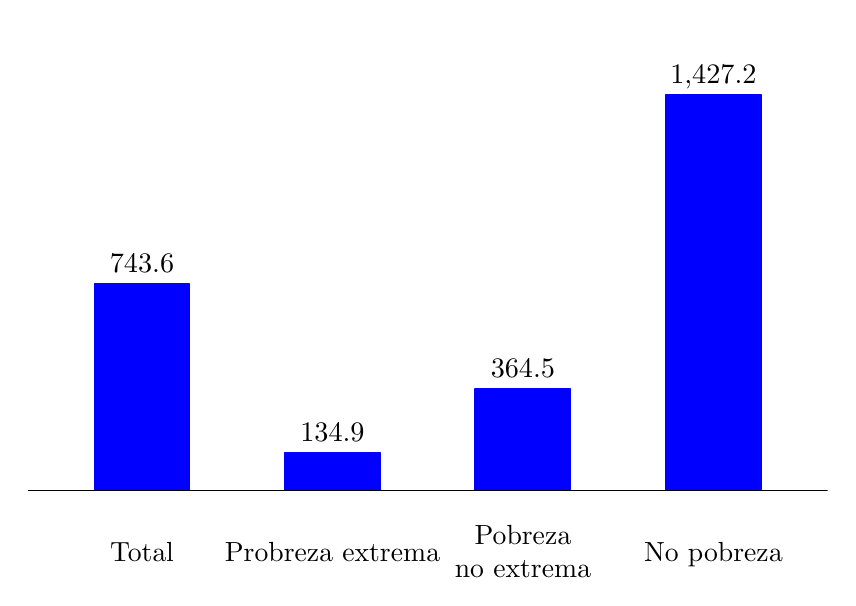
\begin{tikzpicture}[x=1pt,y=1pt]  % Created by tikzDevice version 0.9 on 2016-02-28 22:06:22
% !TEX encoding = UTF-8 Unicode
\definecolor{fillColor}{RGB}{255,255,255}
\path[use as bounding box,fill=fillColor,fill opacity=0.00] (0,0) rectangle (289.08,198.74);
\begin{scope}
\path[clip] (  0.00,  0.00) rectangle (289.08,198.74);

\path[] (  0.00,  0.00) rectangle (289.08,198.74);
\end{scope}
\begin{scope}
\path[clip] (  0.00,  0.00) rectangle (289.08,198.74);

\path[] (  0.00, 24.65) rectangle (289.08,181.67);

\path[] ( 41.30, 24.65) --
	( 41.30,181.67);

\path[] (110.13, 24.65) --
	(110.13,181.67);

\path[] (178.95, 24.65) --
	(178.95,181.67);

\path[] (247.78, 24.65) --
	(247.78,181.67);
\definecolor{drawColor}{RGB}{0,0,255}
\definecolor{fillColor}{RGB}{0,0,255}

\path[draw=drawColor,line width= 0.6pt,line join=round,fill=fillColor] ( 24.09, 31.78) rectangle ( 58.50,106.16);

\path[draw=drawColor,line width= 0.6pt,line join=round,fill=fillColor] ( 92.92, 31.78) rectangle (127.33, 45.28);

\path[draw=drawColor,line width= 0.6pt,line join=round,fill=fillColor] (161.75, 31.78) rectangle (196.16, 68.24);

\path[draw=drawColor,line width= 0.6pt,line join=round,fill=fillColor] (230.58, 31.78) rectangle (264.99,174.53);
\definecolor{drawColor}{RGB}{0,0,0}

\path[draw=drawColor,line width= 0.1pt,line join=round] (  0.00, 31.78) -- (289.08, 31.78);

\node[text=drawColor,anchor=base,inner sep=0pt, outer sep=0pt, scale=  1.02] at ( 41.30,110.13) {743.6};

\node[text=drawColor,anchor=base,inner sep=0pt, outer sep=0pt, scale=  1.02] at (110.13, 49.25) {134.9};

\node[text=drawColor,anchor=base,inner sep=0pt, outer sep=0pt, scale=  1.02] at (178.95, 72.21) {364.5};

\node[text=drawColor,anchor=base,inner sep=0pt, outer sep=0pt, scale=  1.02] at (247.78,178.50) {1,427.2};

\path[] (  0.00, 24.65) rectangle (289.08,181.67);
\end{scope}
\begin{scope}
\path[clip] (  0.00,  0.00) rectangle (289.08,198.74);

\path[] (  0.00, 24.65) --
	(289.08, 24.65);
\end{scope}
\begin{scope}
\path[clip] (  0.00,  0.00) rectangle (289.08,198.74);

\path[] ( 41.30, 21.90) --
	( 41.30, 24.65);

\path[] (110.13, 21.90) --
	(110.13, 24.65);

\path[] (178.95, 21.90) --
	(178.95, 24.65);

\path[] (247.78, 21.90) --
	(247.78, 24.65);
\end{scope}
\begin{scope}
\path[clip] (  0.00,  0.00) rectangle (289.08,198.74);
\definecolor{drawColor}{RGB}{0,0,0}

\node[text=drawColor,anchor=base,inner sep=0pt, outer sep=0pt, scale=  1.00] at ( 41.30,  5.94) {Total};

\node[text=drawColor,anchor=base,inner sep=0pt, outer sep=0pt, scale=  1.00] at (110.13,  5.94) {Probreza extrema};

\node[text=drawColor,anchor=base,inner sep=0pt, outer sep=0pt, scale=  1.00] at (178.95, 11.88) {Pobreza };

\node[text=drawColor,anchor=base,inner sep=0pt, outer sep=0pt, scale=  1.00] at (178.95,  0.00) { no extrema};

\node[text=drawColor,anchor=base,inner sep=0pt, outer sep=0pt, scale=  1.00] at (247.78,  5.94) {No pobreza};
\end{scope}
  \end{tikzpicture}}{Instituto Nacional de Estadística, Encovi 2014.}

\cajita{Gasto en educación por área de residencia}{El gasto en educación de los hogares tiene diferencias según el área de residencia.  En los hogares con residencia en el área rural, la asignación de gasto fue de Q358.5 per capita. Mientras que en el área urbana fue de Q1,136, siendo 3.2 veces mayor que en los hogares en el área rural.}{Gasto promedio per cápita anual en educación por área de residencia}{República de Guatemala, 2014, en quetzales de 2014}{\ \\[0mm]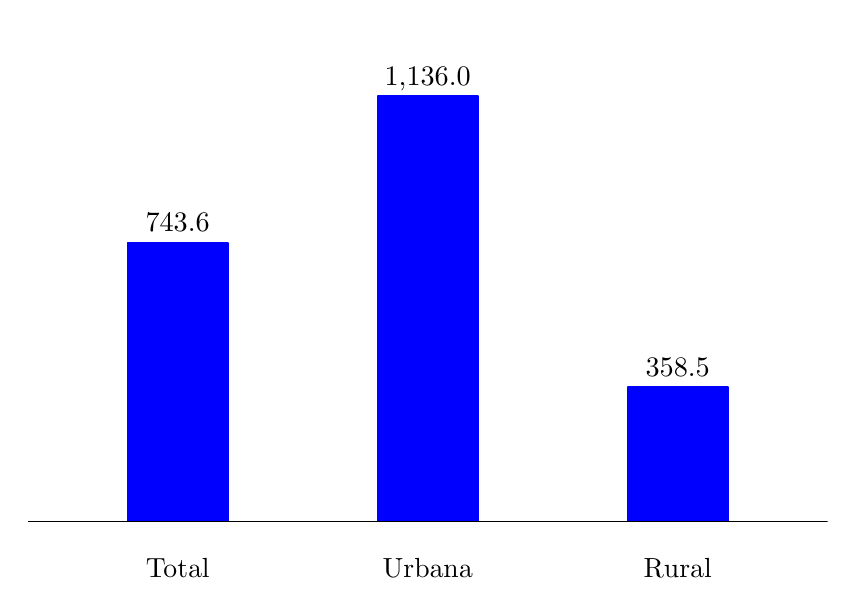
\begin{tikzpicture}[x=1pt,y=1pt]  % Created by tikzDevice version 0.9 on 2016-02-28 22:06:24
% !TEX encoding = UTF-8 Unicode
\definecolor{fillColor}{RGB}{255,255,255}
\path[use as bounding box,fill=fillColor,fill opacity=0.00] (0,0) rectangle (289.08,198.74);
\begin{scope}
\path[clip] (  0.00,  0.00) rectangle (289.08,198.74);

\path[] (  0.00,  0.00) rectangle (289.08,198.74);
\end{scope}
\begin{scope}
\path[clip] (  0.00,  0.00) rectangle (289.08,198.74);

\path[] (  0.00, 12.77) rectangle (289.08,181.67);

\path[] ( 54.20, 12.77) --
	( 54.20,181.67);

\path[] (144.54, 12.77) --
	(144.54,181.67);

\path[] (234.88, 12.77) --
	(234.88,181.67);
\definecolor{drawColor}{RGB}{0,0,255}
\definecolor{fillColor}{RGB}{0,0,255}

\path[draw=drawColor,line width= 0.6pt,line join=round,fill=fillColor] ( 36.13, 20.44) rectangle ( 72.27,120.95);

\path[draw=drawColor,line width= 0.6pt,line join=round,fill=fillColor] (126.47, 20.44) rectangle (162.61,173.99);

\path[draw=drawColor,line width= 0.6pt,line join=round,fill=fillColor] (216.81, 20.44) rectangle (252.95, 68.90);
\definecolor{drawColor}{RGB}{0,0,0}

\path[draw=drawColor,line width= 0.1pt,line join=round] (  0.00, 20.44) -- (289.08, 20.44);

\node[text=drawColor,anchor=base,inner sep=0pt, outer sep=0pt, scale=  1.02] at ( 54.20,124.92) {743.6};

\node[text=drawColor,anchor=base,inner sep=0pt, outer sep=0pt, scale=  1.02] at (144.54,177.96) {1,136.0};

\node[text=drawColor,anchor=base,inner sep=0pt, outer sep=0pt, scale=  1.02] at (234.88, 72.87) {358.5};

\path[] (  0.00, 12.77) rectangle (289.08,181.67);
\end{scope}
\begin{scope}
\path[clip] (  0.00,  0.00) rectangle (289.08,198.74);

\path[] (  0.00, 12.77) --
	(289.08, 12.77);
\end{scope}
\begin{scope}
\path[clip] (  0.00,  0.00) rectangle (289.08,198.74);

\path[] ( 54.20, 10.02) --
	( 54.20, 12.77);

\path[] (144.54, 10.02) --
	(144.54, 12.77);

\path[] (234.88, 10.02) --
	(234.88, 12.77);
\end{scope}
\begin{scope}
\path[clip] (  0.00,  0.00) rectangle (289.08,198.74);
\definecolor{drawColor}{RGB}{0,0,0}

\node[text=drawColor,anchor=base,inner sep=0pt, outer sep=0pt, scale=  1.00] at ( 54.20, -0.00) {Total};

\node[text=drawColor,anchor=base,inner sep=0pt, outer sep=0pt, scale=  1.00] at (144.54, -0.00) {Urbana};

\node[text=drawColor,anchor=base,inner sep=0pt, outer sep=0pt, scale=  1.00] at (234.88, -0.00) {Rural};
\end{scope}
  \end{tikzpicture}}{Instituto Nacional de Estadística, Encovi 2014.}

\cajota{Gasto en educación en los departamentos}{Los departamentos que presentaron mayor gasto per cápita en educación fueron Guatemala (Q1,418.5), Sacatepéquez (Q935.7) y Quetzaltenango (Q920.5).
	
	Los departamentos con menor gasto son: Totonicapán (Q361.3), Huehuetenango (Q371.3) y Sololá (Q400.8).}{Gasto promedio per cápita anual en educación }{Departamental, 2014, en quetzales de 2014}{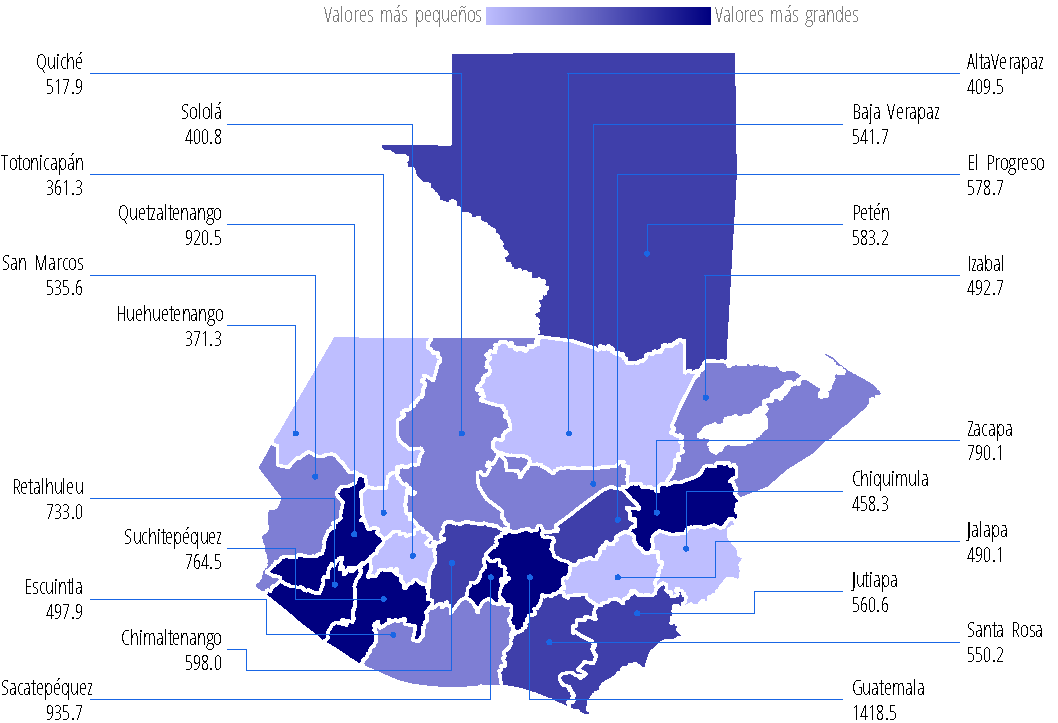
\includegraphics{graficas/GastoHogares/5_07.pdf}}{Instituto Nacional de Estadística, Encovi 2014.}
